\section{Android Mockup}

\begin{tcolorbox}
In diesem Kapitel werden erste Skizzen (Mockups) der Benutzeroberflächen dargestellt.
Diese sollen in erster Linie dazu dienen, dem Kunden einen Überblick über die zu erstellenden UIs zu geben und ggf. Änderungen frühzeitig durchführen zu können.
Dafür eignen sich spezielle Tools, wie z.B. Balsamiq Mockups\footnote{\url{https://balsamiq.com/products/mockups}}.
\end{tcolorbox}


\begin{figure}[h]
\begin{tabularx}{\textwidth}{X  X}
	\includegraphics[scale = 0.155]{img/AndroidMockup/splash}  \caption {Startbildschirm} &  Dies ist der Startbildschirm \\
	\includegraphics[scale = 0.155]{img/AndroidMockup/login} \caption {Login Bildschirm} &	Nachdem man auf dem Startbildschirm auf 'Login' gedrückt hat, landet man auf dem Anmeldebildschirm. Hier hat man die Möglichkeit sich anhand der Kundennummer und dem Passwort einloggen. Außerdem hat man die Möglichkeit sich mithilfe von dem 'Passwort vergessen' Button sich sein Passwort zuschicken zu lassen. \\ 
\end{tabularx}
\end{figure}


\begin{figure}[h]
\begin{tabularx}{\textwidth}{X  X}
	\includegraphics[scale = 0.155]{img/AndroidMockup/forgotPassword} \caption{Password vergessen} & Nachdem man auf 'Passwort vergessen' geklickt hat, erscheint eine Meldung mit 'Ihr Passwort wurde an ihre Email gesendet' und das Passwort wird an die zu der Kundennummer gehörigen Email-Adresse geschickt. \\
	\includegraphics[scale = 0.155]{img/AndroidMockup/Main} \caption{Startbildschirm} & Nachdem man sich erfolgreich eingeloggt hat, landet man auf dem Startbildschirm. Hier sieht man eine Übersicht über seine Zählerstände mit Zählernummer sowie den aktuellen Zählerstand des jeweiligen Zählers. \\
\end{tabularx}
\end{figure}


\begin{figure}[h]
\begin{tabularx}{\textwidth}{X  X}
	\includegraphics[scale = 0.155]{img/AndroidMockup/FABMenu} \caption{FABMenü}  & Klickt man auf den Button unten rechts, erscheint ein Dropdown Menü. Hier kann man sich entscheiden ob man ein Bild live aufnehmen möchte (Kamera Symbol) oder ein Bild eines Zählers aus der Galerie hochladen möchte(Galerie Symbol). \\
	\includegraphics[scale = 0.155]{img/AndroidMockup/SystemCamera} \caption{Kamera-View}  & Nachdem man im Dropdown Menü das Kamera Symbol gedrückt hat, öffnet sich die integrierte Kamera App und man kann den Zähler abfotografieren.  \\ 
\end{tabularx}
\end{figure}

\begin{figure}[h]
\begin{tabularx}{\textwidth}{X  X}
	\includegraphics[scale = 0.155]{img/AndroidMockup/imageFailed} \caption{Scan Fehlgeschlagen} & Wurde auf dem Bild kein Zähler erkannt, so erscheint eine Popup Benachrichtung mit 'Scan nicht erfolgreich'. Hier hat man die Möglichkeit erneut ein Foto zu machen oder den Vorgang abzubrechen. \\
	\includegraphics[scale = 0.155]{img/AndroidMockup/check} \caption{Werte überprüfen} & Wurde erfolgreich der Zähler abfotografiert, so folgt eine Überprüfung der Zahlen welche Azure erkannt hat. Diese Zahlen muss man Bestätigen bevor sie eingetragen werden. \\ 
\end{tabularx}
\end{figure}

\begin{figure}[h]
\begin{tabularx}{\textwidth}{X  X}
	\includegraphics[scale = 0.155]{img/AndroidMockup/illegalFormatException} \caption{Falsches Zahlenformat} & Gibt man beim Zählerstand ein falsches Zahlenformat ein, so erhält man die Meldung 'Ungültiges Format: Der Zählerstand besteht aus ..  Ziffern'.  Da verschiedene Zähler, verschiedene Zahlenformate besitzen ist die Lücke der Ziffern variable und wird je nach Zähler variable angepasst.   \\
	\includegraphics[scale = 0.155]{img/AndroidMockup/history} \caption{Zählerstand History} & Klickt man auf einen der Zähler, so sieht man die ganze History der Zählerstände. Außerdem sieht man wann der Zählerstand hochgeladen worden ist und ob es per manuelle Eingabe oder per Foto aufgenommen wurde. \\
\end{tabularx}
\end{figure}

\begin{figure}[h]
\begin{tabularx}{\textwidth}{X  X}
	\includegraphics[scale = 0.155]{img/AndroidMockup/manuelEntry} \caption{Manueller Eintrag}&  Klickt man nachdem auf einen Zähler geklickt hat, auf manuelle Eingabe, so hat man die Möglichkeit den Zählerstand manuell einzutragen.  \\
	\includegraphics[scale = 0.155]{img/AndroidMockup/rename} \caption{Offline-Meldung} & Verliert man in einem Vorgang die Internet verbindung, so erscheint eine Meldung mit 'Du bist offline' und der Vorgang wird nicht durchgeführt.  \\ 
\end{tabularx}
\end{figure}

\begin{figure}[h]
\begin{tabularx}{\textwidth}{X  X}
	\includegraphics[scale = 0.155]{img/AndroidMockup/serverException} \caption{Serverfehler} & Verliert man in einem Vorgang die Verbindung zum Server oder es liegen Probleme beim Server vor, erscheint eine Meldung mit 'Serverfehler: Bitte versuche es erneut' und der Vorgang wird nicht durchgeführt. \\
	\includegraphics[scale = 0.155]{img/AndroidMockup/correct} \caption{Zählerstand korregieren} & Hat man einen Zählerstand falsch eingetragen, hat man nachträglich die Möglichkeit den Zählerstand manuell anzupassen. \\ 
\end{tabularx}
\end{figure}

\begin{figure}[h]
\begin{tabularx}{\textwidth}{X  X}
	\includegraphics[scale = 0.155]{img/AndroidMockup/dropdown} \caption{Dropdown Menü} & Man hat auf dem Startbildschirm außerdem die Möglichkeit oben rechts ein kleines Dropdown-Menü zu öffnen. Hier hat man die Möglichkeit die Adresse des Servers auszuwählen sowie eine Nachricht an den Support zu schreiben. (Kontakt) \\
	\includegraphics[scale = 0.155]{img/AndroidMockup/contact} \caption{Kontakformular} & Möchte man eine Nachricht an den Support schreiben, so klickt man auf 'Kontakt' und landet auf dem Kontaktformular. Hier muss man seinen Namen, seine Email, den Betreff sowie die gewünschte Nachricht angeben. \\ 
\end{tabularx}
\end{figure} 

\begin{figure}[h]
\begin{tabularx}{\textwidth}{X  X}
	\includegraphics[scale = 0.155]{img/AndroidMockup/serverLocation} \caption{Server wählen} & Möchte man die Adresse des Servers ändern, so klickt man auf 'Server wählen'. Hier hat man jetzt die Möglichkeit den Servers mithilfe der Server IP Adresse zu bestimmen und zu wechseln.
\end{tabularx}
\end{figure}

% OwO Section Web OwO

\newpage

\begin{figure}[h] 
	\newpage
	\section{Web Mockup}
	\centering
    \includegraphics[scale=0.3]{img/WebsiteMockup/Login-User}
	\caption{Login Bildschirm} \hfill \break
	Hier sieht man den Login Screen in dem sich User und Admins mithilfe von Kundennummer und Passwort anmelden kann.
\end{figure}
 
\newpage

\begin{figure}[h]
	\centering
    \includegraphics[scale=0.3]{img/WebsiteMockup/Dashboard-User-NonSelected}
	\caption{Dashboard User} \hfill \break
	Nachdem man sich erfolgreich eingeloggt wird man auf den Startbildschirm weitergeleitet. Hier kann der Benutzer seine Zähler einsehen.
\end{figure}

\newpage

\begin{figure}[h]
	\centering
    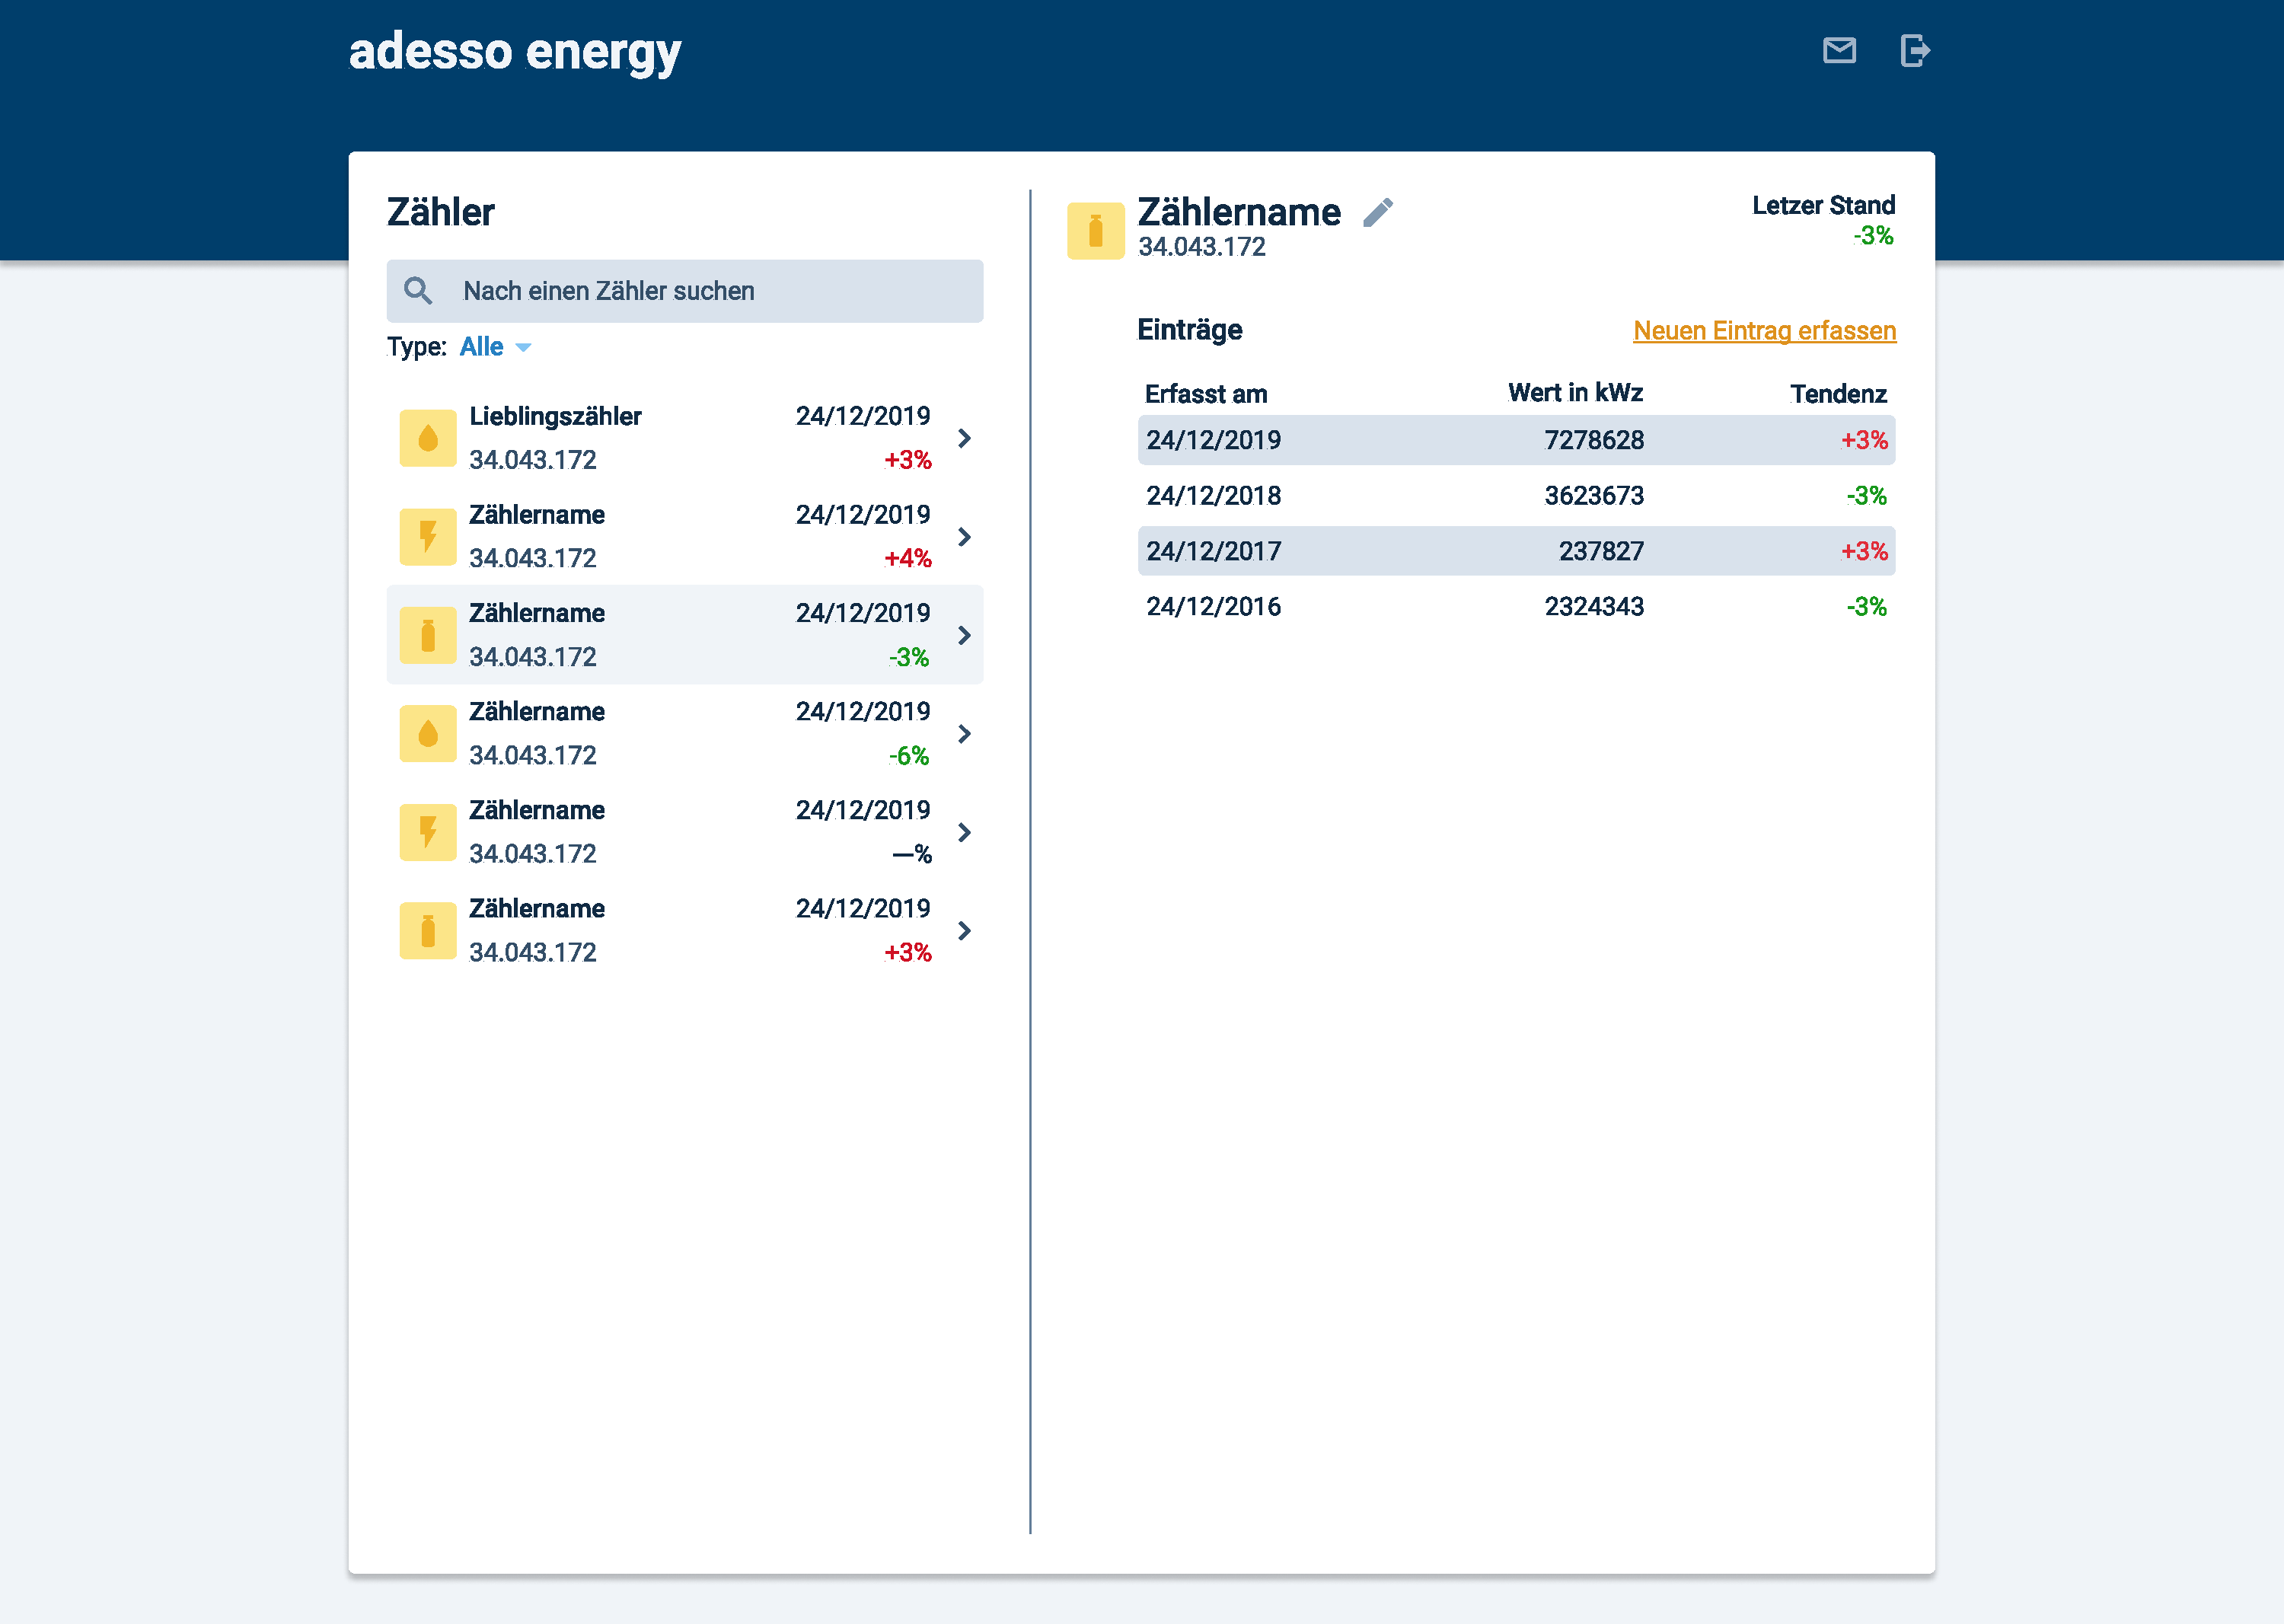
\includegraphics[scale=0.3]{img/WebsiteMockup/Dashboard-User-Selected}
	\caption{Dashboard User mit ausgewähltem Zähler} \hfill \break
	Nachdem man einen Zähler ausgewählt hat, sieht man seine History mit Datum und Zählerstand.
\end{figure}

\newpage

\begin{figure}[h]
	\centering
    \includegraphics[scale=0.3]{img/WebsiteMockup/Dashboard-User-Selected-AddEntry}
	\caption{Dashboard User Eintrag hinzufügen} \hfill \break
	Nachdem man auf Neuen Eintrag erfassen klickt, wird ein Dialog angezeigt um einen neuen Stand festzuhalten.
\end{figure}

\newpage

\begin{figure}[h]
	\centering
    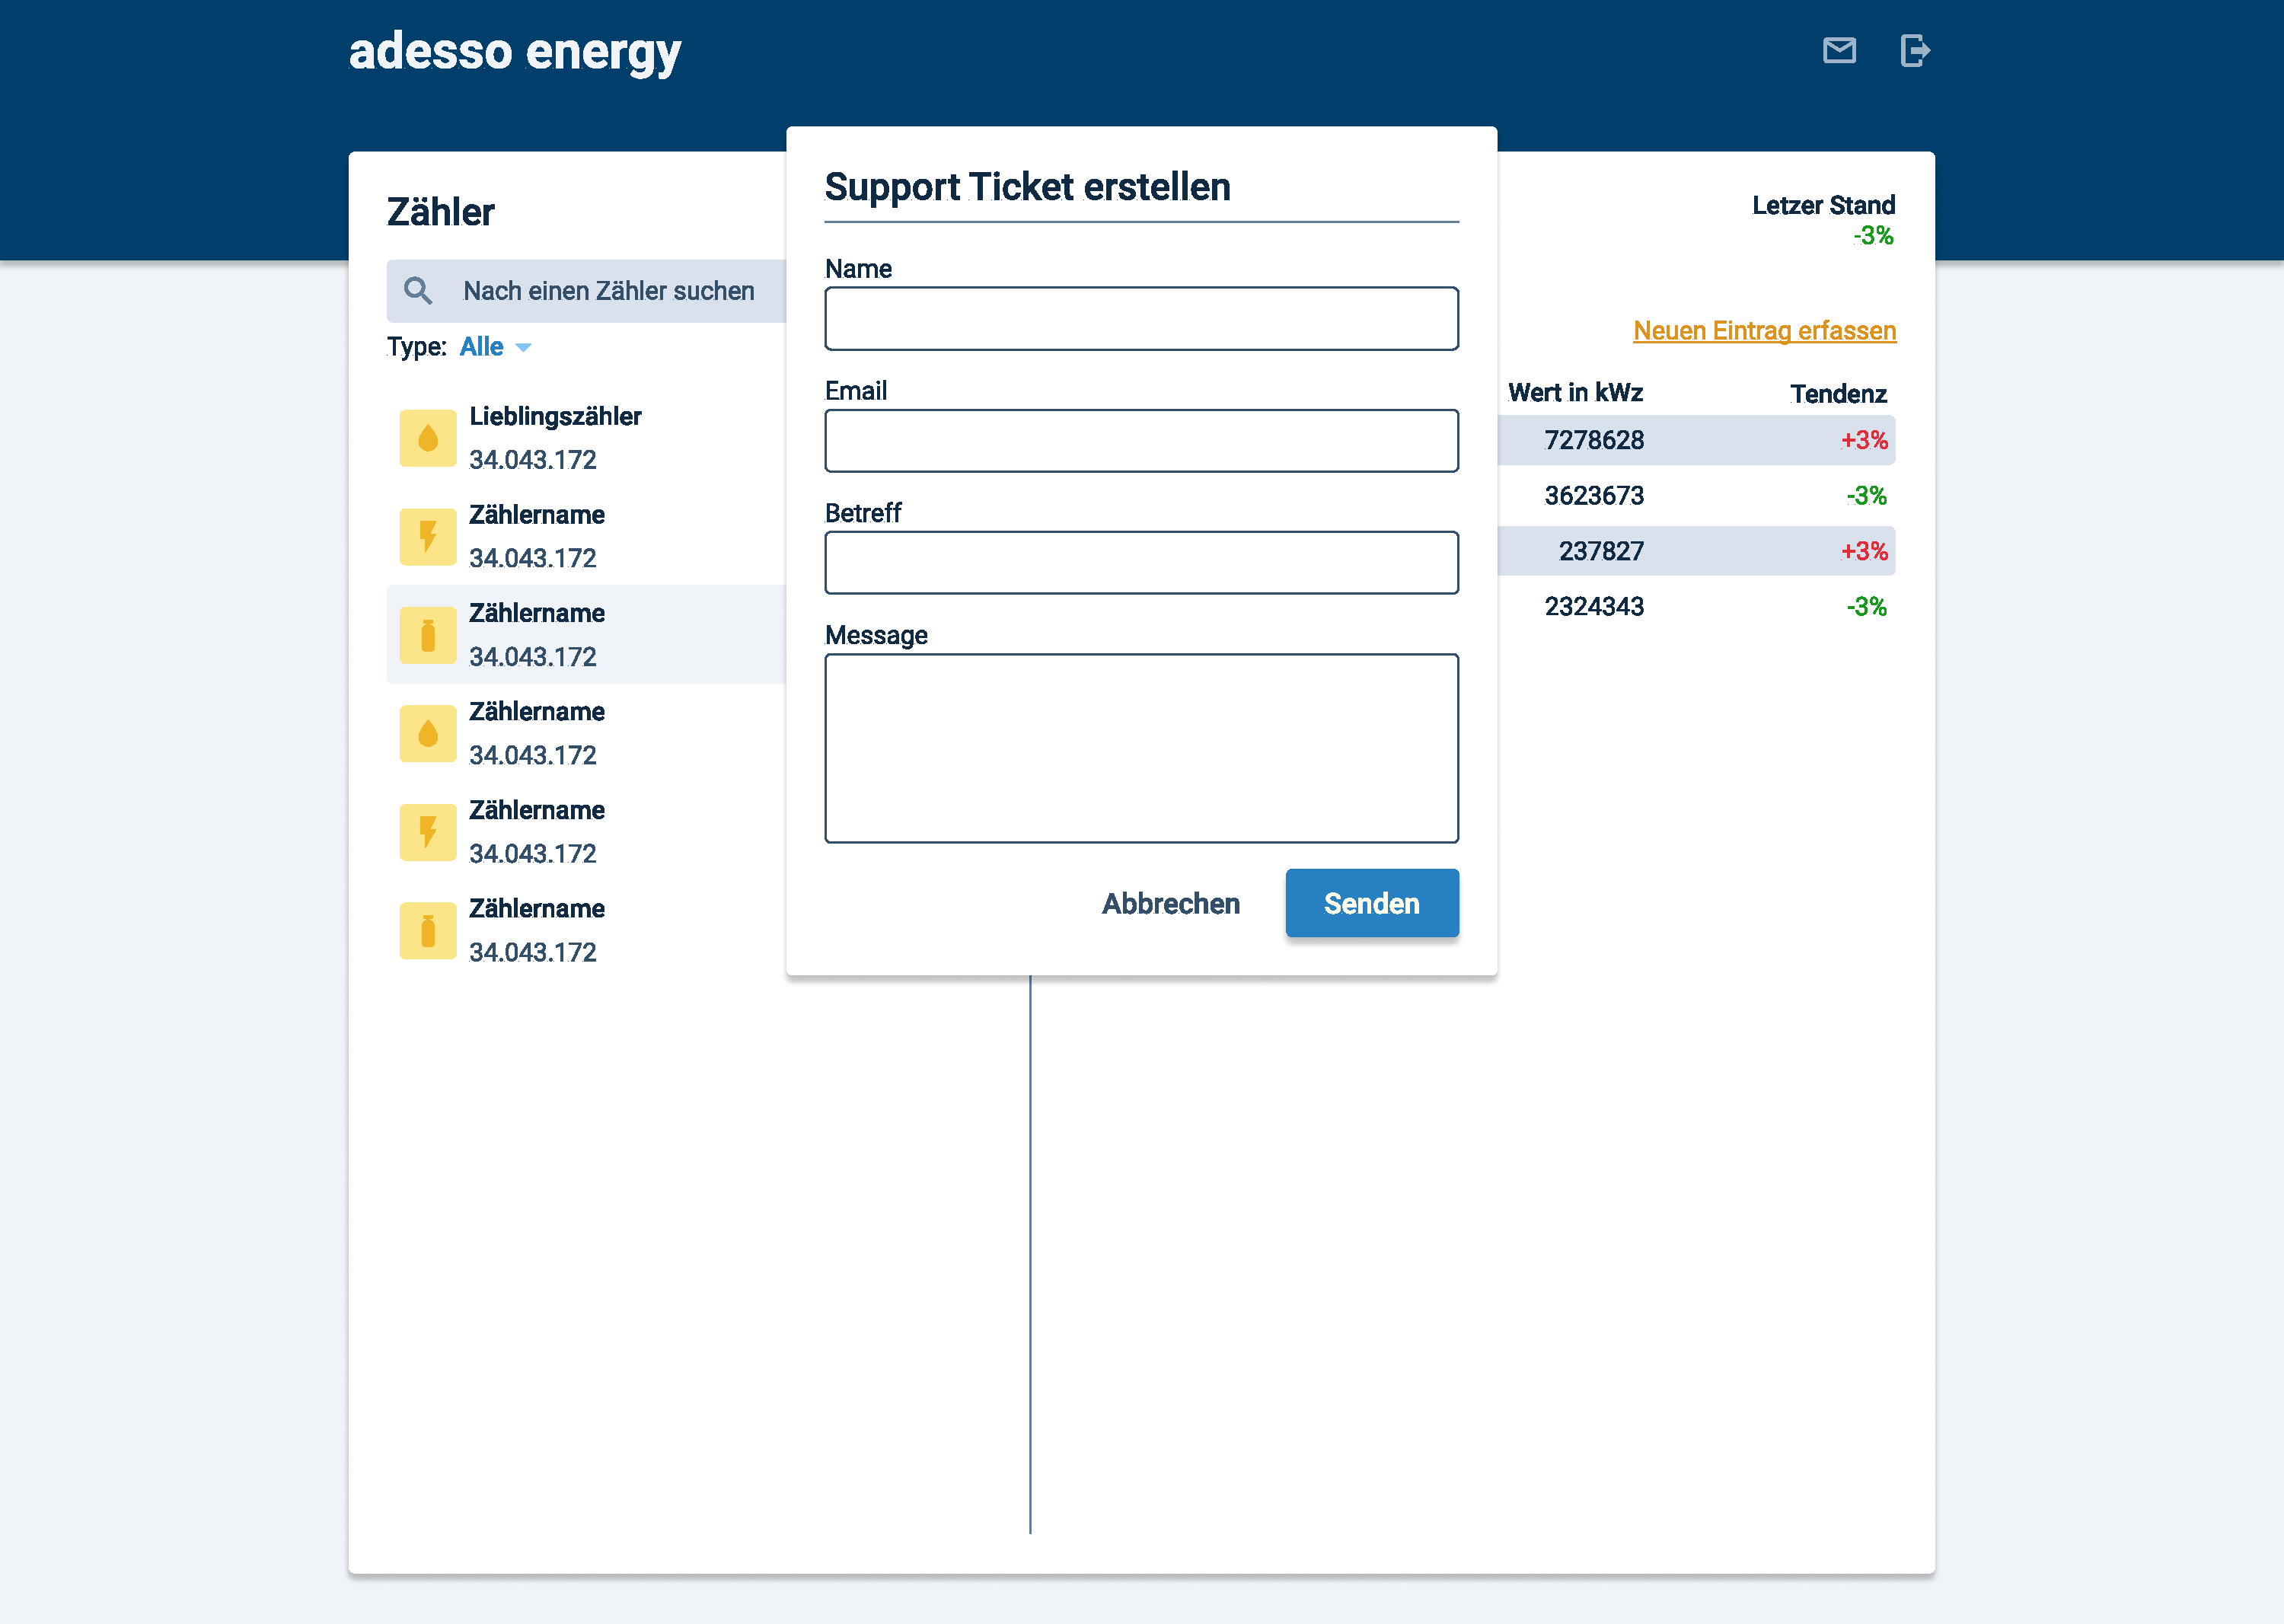
\includegraphics[scale=0.3]{img/WebsiteMockup/Dashboard-User-Mail}
	\caption{Dashboard User Support} \hfill \break
	Durch klicken auf das Mail Icon oben rechts auf der Seite wird ein Dialog zum erstellen eines neuen Support Tickets angezeigt.
\end{figure}

\newpage

\begin{figure}[h]
	\centering
    \includegraphics[scale=0.3]{img/WebsiteMockup/Dashboard-Admin-NonSelected}
	\caption{Dashboard Admin} \hfill \break
	Nachdem Login hat ein Administrator die Möglichkeit alle Kunden einzusehen.
\end{figure}

\newpage

\begin{figure}[h]
	\centering
    \includegraphics[scale=0.3]{img/WebsiteMockup/Dashboard-Admin-UserSelected}
	\caption{Dashboard Admin Benutzer ausgewählt} \hfill \break
	Nachdem der Administrator einen Kunden ausgewählt hat kann er die Informationen des Kunden einsehen.
\end{figure}

\newpage

\begin{figure}[h]
	\centering
    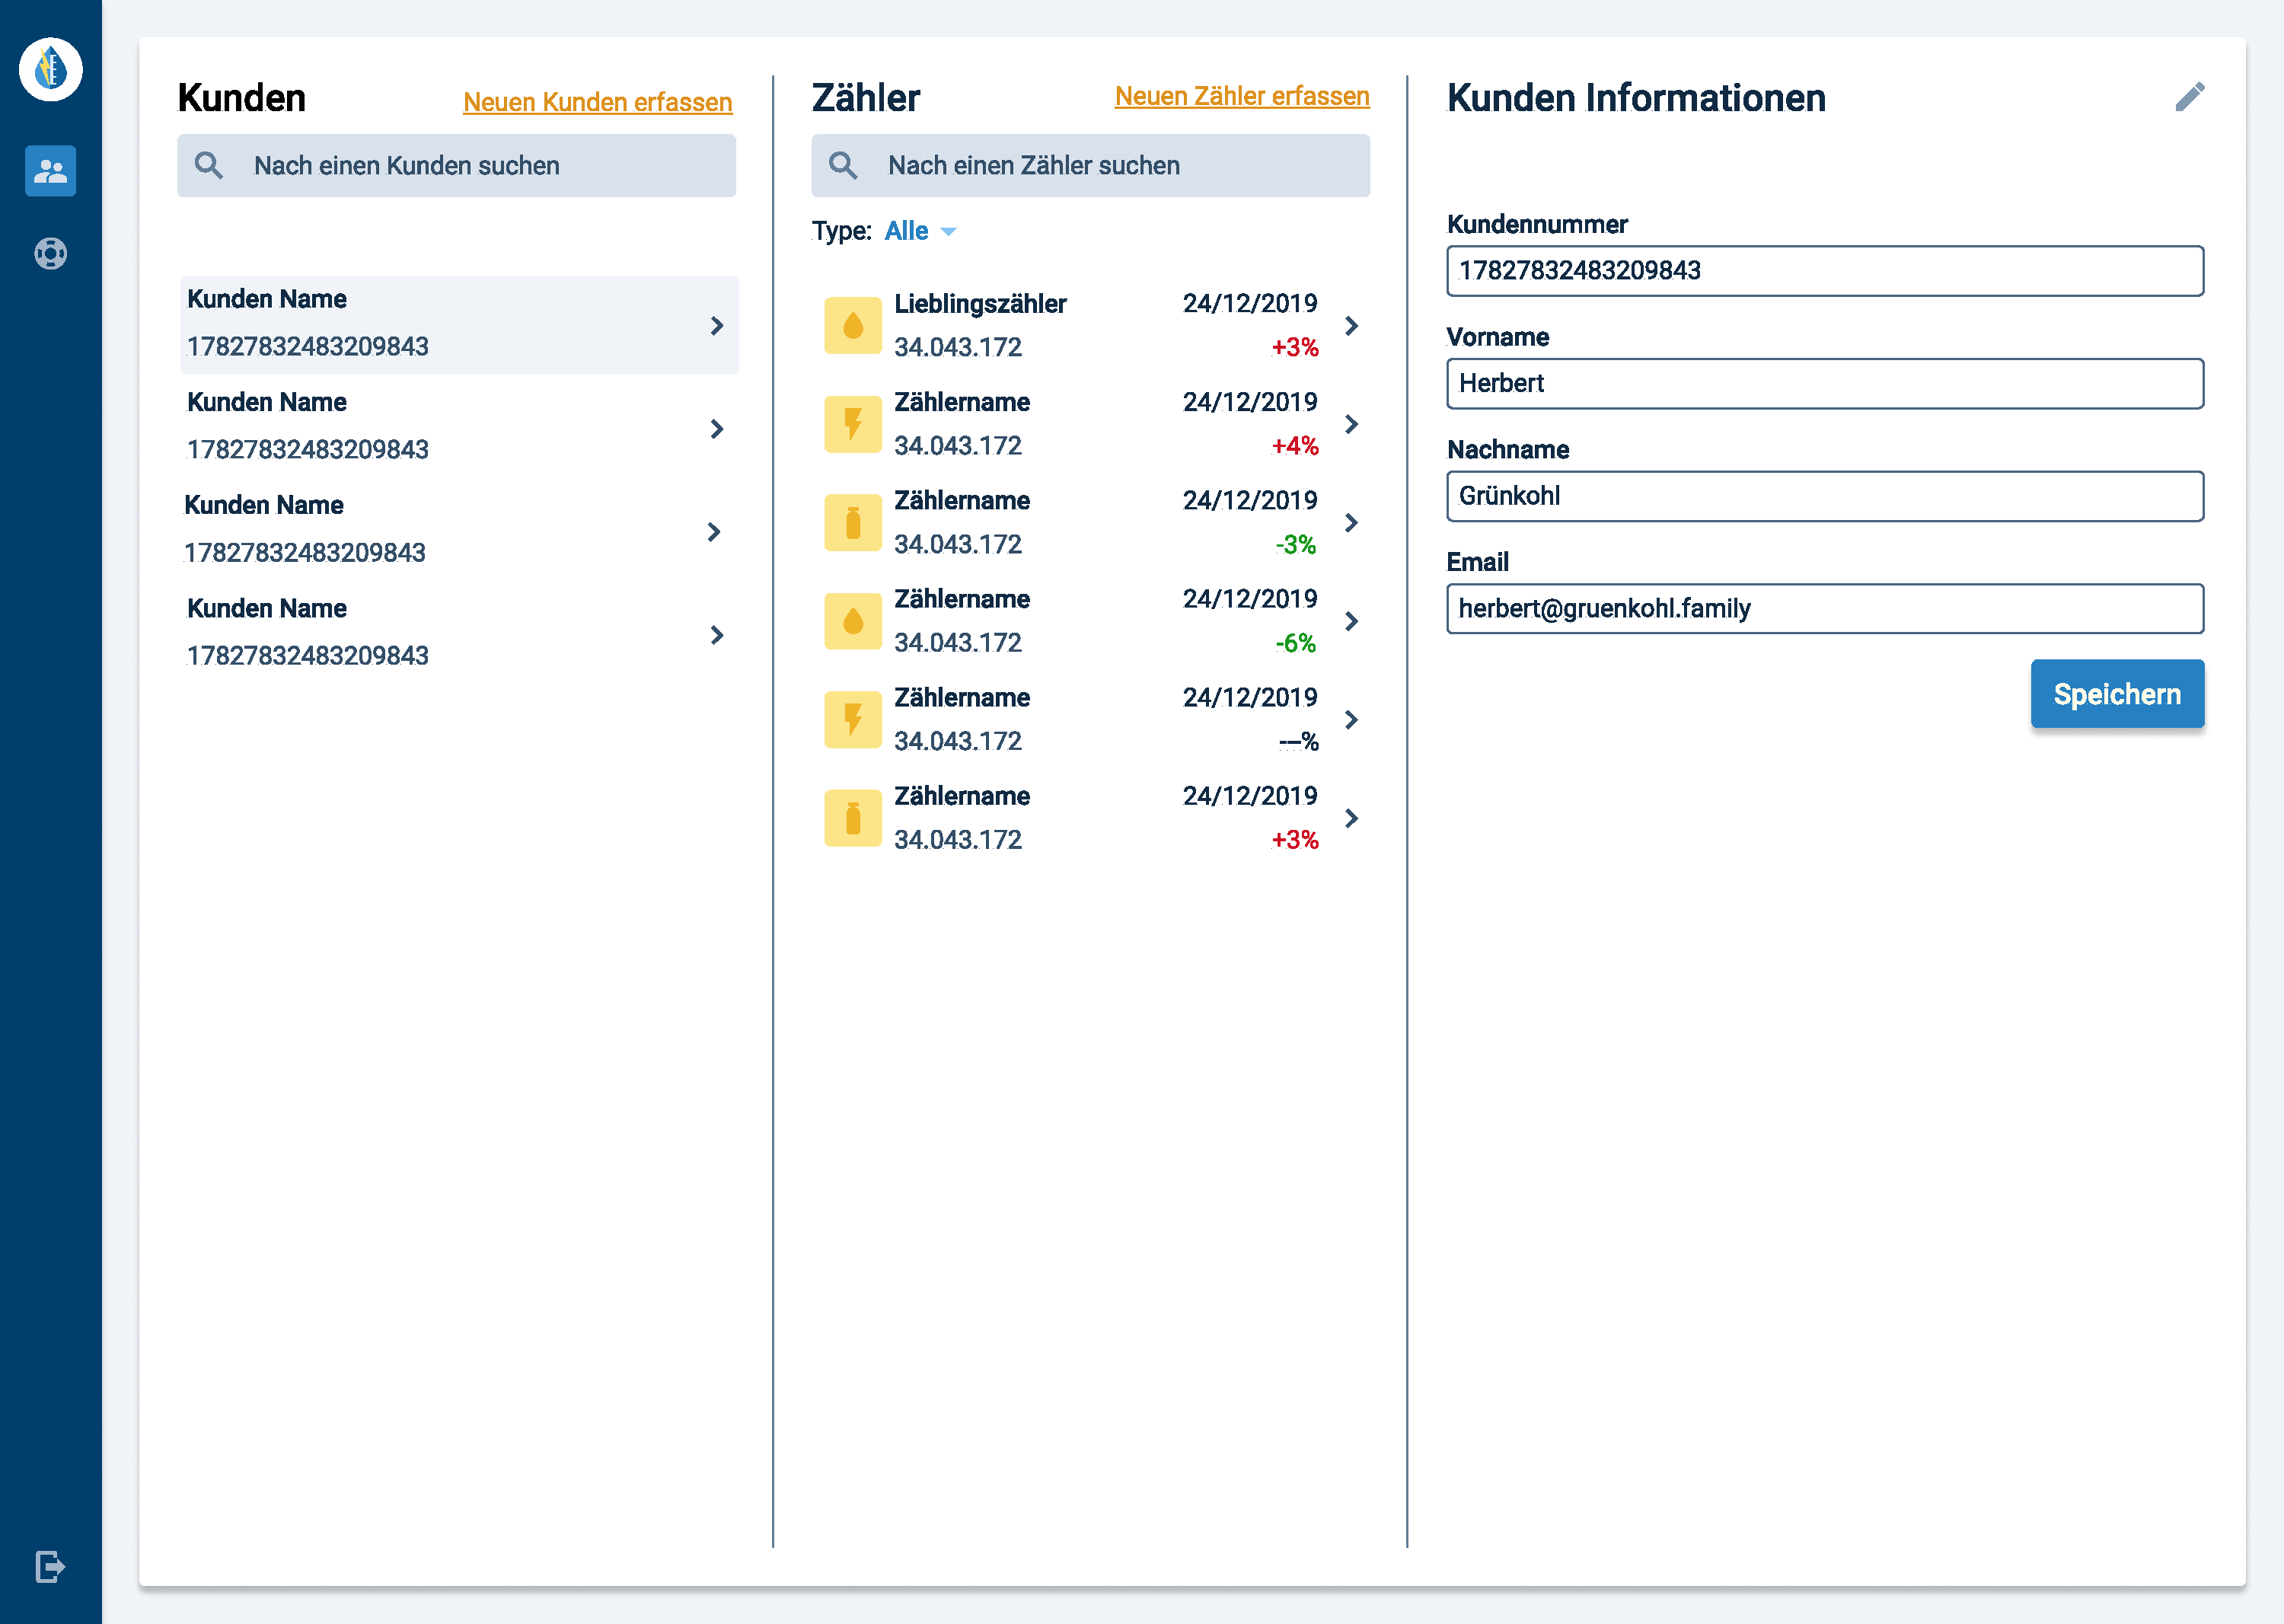
\includegraphics[scale=0.3]{img/WebsiteMockup/Dashboard-Admin-UserSelected-Edit}
	\caption{Dashboard Admin Benutzer editieren}\hfill \break
	Durch klicken des Stift Icons oben rechts auf der Seite kann ein Administrator den ausgewählten Kunden bearbeiten.
\end{figure}
\newpage

\begin{figure}[h]
	\centering
    \includegraphics[scale=0.3]{img/WebsiteMockup/Dashboard-Admin-AddUser}
	\caption{Dashboard Admin Benutzer hinzufügen} \hfill \break
	Durch klicken auf Neuen Kunden erfassen kann der Administrator einen neuen Kunden zur Datenbank hinzufügen.
\end{figure}

\newpage

\begin{figure}[h]
	\centering
    \includegraphics[scale=0.3]{img/WebsiteMockup/Dashboard-Admin-AddZahler}
	\caption{Dashboard Admin Zähler hinzufügen} \hfill \break
	Nachdem der Administrator einen Benutzer ausgewählt hat, kann er diesem einen neuen Zähler hinzufügen, indem er auf Neuen Zähler erfassen klickt.
\end{figure}

\newpage

\begin{figure}[h]
	\centering
    \includegraphics[scale=0.3]{img/WebsiteMockup/Dashboard-Admin-ZahlerSelected}
	\caption{Dashboard Admin Zähler ausgewählt} \hfill \break
	Nachdem der Adnimistrator auf einen Zähler geklickt hat, sieht er die Zählerinformation und History.
\end{figure}

\newpage

\begin{figure}[h]
	\centering
    \includegraphics[scale=0.3]{img/WebsiteMockup/Dashboard-Admin-AddEntry}
	\caption{Dashboard Admin Eintrag hinzufügen} \hfill \break
	Wie auch der Benutzer hat der Admin auch die Möglichkeit Zählerstände einzutragen.
\end{figure}

\newpage

\begin{figure}[h]
	\centering
    \includegraphics[scale=0.3]{img/WebsiteMockup/Dashboard-Admin-Support}
	\caption{Dashboard Admin Support} \hfill \break
	Nach dem klicken auf das Support Icon am linken Rand der Seite kann ein Administrator alle offenen Support Tickets einsehen.
\end{figure}

\newpage

\begin{figure}[h]
	\centering
    \includegraphics[scale=0.3]{img/WebsiteMockup/Dashboard-Admin-Support-Selected}
	\caption{Dashboard Admin Support Ticket ausgewählt} \hfill \break
	Durch auswählen einen Tickets kann der Administrator alle Information über das Ticket einsehen, das Ticket schließen, oder Rückfragen stellen.
\end{figure}

